%To accomplish the goals 

%This chapter will illuminate the details of how encryption, authentication, network coding, and ARQ management are implemented in the network
%interfaces.

%Recall that the architecture of a \gls{noc} consists of a router grid with each node connected to a local processing element through a network
%interface (cf. Figure \vref{fig:nocexample}). The 

Over the course of this chapter, the design of the communication protocol in all variants will be thorougly explained. To begin, fundamental
assumptions about the environment and basic building blocks of the protocol are presented. Since the protocol variants share many elements and differ
mostly in the authentication scheme, the simplest one (uncoded individual authentication) is used to give a step-by-step explanation of the full
protocol. Following this, the other variants are described by drawing upon the differences to uncoded individual authentication.

\section{Design Aspects}
\subsection{Unicast And Multicast}
In Section \ref{sec:assandsig}, it was already hinted that this thesis concerns itself with the unicast communication pattern. In this scenario, each
flit is sent to a single specified destination. In contast, multicast facilitates the existance of multiple receivers for a single flit.

While there has been notable work on \gls{noc} multicast protocols, especially in conjuction with network coding, this thesis builds directly upon
research in the unicast domain (cf. Section \ref{sec:ncfornoc}). Hence, multicast will not be considered for the implementation, experiments, and
evaluation performed here.

\subsection{Flit Structure}\label{subsec:flitstructure}
As mentioned in Section \ref{sec:flitsfun}, flits are the fundamental unit of transmission for this thesis. They contain several header fields and a
payload. Their structure differs slightly depending on whether or not network coding is employed. For network coded flits, one additional
header field is required (the global encoding vector) and the generation ID replaces the flit ID. This structure is depicted in Figure
\vref{fig:flitstructureuncoded} (uncoded) and Figure \ref{fig:flitstructurenetworkcoded} (network coded).
% TODO: table comparing the protocol variants, their properties (e.g. lane width)

\begin{figure}
    \centering
    \includegraphics[width=\textwidth]{flit-structure-uc}
    \caption[The structure of a flit without network coding]{The structure and data layout of a flit in an environment without network coding
    (uncoded). The fixed size of the header fields and the payload results in an invariant total size of 141 bit.}
    \label{fig:flitstructureuncoded}
\end{figure}

\begin{figure}
    \centering
    \includegraphics[width=\textwidth]{flit-structure-nc}
    \caption[The structure of a flit with network coding]{The structure and data layout of a flit in a network coded environment. The fixed size of
    the header fields and the payload results in an invariant total size of 149 bit.}
    \label{fig:flitstructurenetworkcoded}
\end{figure}

The header fields are required for routing the flits to their destinations and for correct processing by the receivers, while the payload carries the
transmitted information. Uncoded flits have the following fields:
\begin{itemize}
    \item \textbf{Burst.} The burst bit is used to indicate an uninterrupted stream of flits between the same sender and receiver. For example, when a
        larger packet is being broken down into multiple flits, the burst bit can be used to indicate the beginning of a flit stream, allowing the
        intermediate routers on the path to the receiver to adjust their routing behavior accordingly in order to minimize stream interruptions. In
        this thesis, however, the burst bit is unused. As there are plans to build upon this work and explore burst configurations, it is still
        included for documentation purposes.
    \item \textbf{Source X, Source Y.} Recalling that the topology of the \gls{noc} is a 2D mesh, the usage of 2D cartesian coordinates to uniquely
        identify nodes suggested itself. Here, zero-based X and Y indices indicate the column and row of a node, respectively. Each field is 4 bit long,
        resulting in at most $16 \cdot 16 = 256$ nodes being addressable. Hence, the maximum \gls{noc} size is \textit{16x16} as well, which is deemed
        sufficient\footnote{It is certainly possible to increase the field sizes to, e.g., 8 bit, allowing for up to $256 \cdot 256 = 65536$ addressable
        nodes, should the need arise. However, as this would increase the flit size, it is not implemented here.}. The source header fields describe
        the address of the flit's sender.
    \item \textbf{Destination X, Destination Y.} These fields also describe the address of a node in 2D cartesian coordinates. As opposed to the
        source fields, they indicate the intended destination of the flit.
    \item \textbf{Mode.} The mode field indicates what type of data the flit contains. It signals to the receiver whether the flit contains, e.g.,
        data, a \gls{mac}, or an \gls{arq}. There are a few more special modes that are explained in Section \ref{sec:theprotocol}. The
        field size is 4 bit, allowing for 16 different modes. Not all of them are used for this thesis, so it is possible to define additional modes
        in a future work if necessary.
    \item \textbf{Address.} This field may contain a 32 bit memory address. In case the flit payload needs to be read from or written to memory, it
        indicates the location of the data. Since this is only relevant to the processing elements and not the network interfaces, the field remains
        unused for this thesis. Nevertheless, it is included in the flits since it affects their size.
    \item \textbf{Flit ID.} The flit ID is a 24 bit numeric identifier. Starting at zero, the IDs are incremented as more flits are generated.
        Similar to sequence numbers (e.g., as employed in \gls{tcp}), they are used to ensure that all flits arrive at the destined processing
        elements in order. Furthermore, it is used to associate related flits. For instance, an encrypted data flit and the corresponding \gls{mac}
        flit have the same ID to express their correlation.
    \item \textbf{Payload.} The payload carries the actual data that are transmitted with a flit. Its size is 64 bit as this is a common plaintext
        size for block ciphers, such as the one used for this thesis, PRINCE \cite{borghoff12prince}.
\end{itemize}
\vspace{0.5\baselineskip}

When network coding is applied to a flit, the following fields are added:
\begin{itemize}
    \item \textbf{Generation ID.} Replacing the flit ID, the generation ID is also a 24 bit numeric idenfier. As network coding intermingles multiple
        flits, their original IDs become meaningless and are replaced by the generation ID (which is the same for all flits of a generation). Apart
        from this, they follow the same rules as the flit IDs described above.
    \item \textbf{Global Encoding Vector.} This field contains the global encoding vector used to create the flit when applying network coding. It is
        required for the receiver to successfully decode a generation and obtain the original flits. Furthermore, since all flits in a generation have
        the same ID, it is used to distinguish between those flits. As with flit IDs in an uncoded setting, corresponding flits (like data and
        \gls{mac}) are associated by having the same \gls{gev} in addition to the same generation ID.
\end{itemize}
\vspace{0.5\baselineskip}

With a size of 141 or 149 bit, respectively, flits are relatively small. While this entails that each one carries comparatively little
information\footnote{The combined size of the header fields (77 or 85 bit, respectively) exceeds the size of the payload (64 bit) considerably.}, it
has the significant advantage that flits can be transferred between directly connected components in a single clock
cycle. For example, sending a flit from a router to a neighboring one, or sending it from a processing element
to the attached network interface takes one cycle. In a hardware implementation, this is facilitated by parallel communication channels that are able
to transmit multiple bits simultaneously. This results in multiple wires (or other electical conductors) at the physical layer, as each one may convey
precisely one bit of information per cycle \cite{wikiparallelcomm}. Thus, for uncoded flits, a channel width of 141 or more wires is required, and at least 149
in a network coded setting.

\subsection{Cryptography}
\begin{itemize}
    \item Encrypt-then-MAC vs. Encrypt-and-MAC (bei Encrypt-then-MAC encrypt+authenticate sequentiell, aber decrypt+verify parallel.
        Bei Encrypt-and-MAC encrypt+authenticate parallel, aber decrypt+verify sequentiell). Bei Encrypt-and-MAC: decrypt kann schon
        beginnen, wenn MAC noch nicht da ist, verringert die Latenz in manchen Fällen.
\end{itemize}

\subsubsection{Notation}
This section introduces formal notations and definitions regarding the cryptographic primitives. They will be used throughout this chapter to
illustrate how flits are processed. They are denoted by variables and functions, where
\begin{itemize}
    \item $p$ is a plaintext message (usually the flit payload),
    \item $c$ is a ciphertext,
    \item $m$ is a \gls{mac},
    \item $k$ is a key (with $k_e$ and $k_m$ referring to encryption and \gls{mac} keys),
    \item $f$ is a complete flit (header and payload),
    \item $e_k(p)$ is an encryption function that takes a plaintext $p$ and produces a ciphertext $c$ using key $k$,
    \item $d_k(c)$ is a decryption function that takes a ciphertext $c$ and produces the plaintext $p$ using key $k$,
    \item $a_k(f)$ is an authentication function that takes a flit and produces a \gls{mac} $m$ using key $k$.
\end{itemize}
\vspace{0.5\baselineskip}

While the functions $e_k(p)$ and $d_k(c)$ take a 64 bit long text as their argument (which matches the cipher's block size), the authentication
function $a_k(f)$ is applied to complete flits, exceeding the block size. Therefore, $a_k(f)$ applies the cipher in conjunction with the \gls{cbcmac}
mode of operation as explained below.

\subsubsection{Drawbacks}
The integration of cryptographic operations inevitably entails a degradation of the network performance which manifests itself in higher transmission
latencies and increased chip area requirements. There usually is a reversely proportional relation between performance and safety: as the level of security
increases, the communication performance declines. In order to satisfy the protection goals of confidentiality and integrity, both encryption and
authentication are required\footnote{Depending on the use case, it may be adequate to fulfill only one of these goals (or none at all), alleviating
the performance drop caused by the security measures. For instance, a preceding work of this thesis concerns itself with providing only integrity in
\glspl{noc} \cite{moriam18activeattackers}.}, resulting in a noticeable performance impact. In order to minimize these effects, several countermeasures
are implemented:
\begin{itemize}
    \item \textbf{Parallel modules.} As the cryptographic computations are the operations with the highest latency in the network interfaces, they
        threaten to become a bottleneck and congest the traffic flow. To prevent this, multiple cryptographic modules are employed in each network
        interface. While this does not speed up the cryptographic computations, it allows for multiple flits to be processed in parallel. For
        instance, each network interface could have three encryption modules, allowing it to encrypt up to three flits simultaneously. Alas, this
        approach naturally increases the occupied chip area.
    \item \textbf{Hardware-optimized ciphers.} In Section \ref{sec:lightweightcrypto}, it was already mentioned that conventional block ciphers, such
        as \gls{aes}, are not efficient enough for usage in \glspl{noc}, in terms of both latency and chip area. However, there is a plethora of
        algorithms specifically designed for an efficient hardware implementation. In the work directly preceding this thesis, they were evaluated and
        compared \cite{harttung17lightweightcrypto}. The most promising algorithm is PRINCE \cite{borghoff12prince}, which is introduced below.
    \item \textbf{Parallel decryption and verification.} When flits arrive from the network, the \gls{mac} is verified to ensure integrity. When
        successful, the data are decrypted and passed on. To speed up this process, verification and decryption is performed in parallel. Should the
        integrity check fail, the decrypted data have to be discarded. In case of success, however, this results in a significant latency reduction.
        This scheme is illustrated in detail in the step-by-step description of the protocol (Section \ref{sec:theprotocol}).
\end{itemize}

\subsubsection{Composition Methods}
The ordering of encryption and authentication (i.e., \gls{mac} computation) has a significant impact on both the achievable performance and the
security of the scheme. There are three general approaches to bring them together \cite{bellare00authenc}:
\begin{itemize}
    \item \textbf{Encrypt-and-MAC.}
    \item \textbf{MAC-then-encrypt.}
    \item \textbf{Encrypt-then-MAC.}
\end{itemize}

\subsubsection{PRINCE}
The cipher that is used for encryption, decryption, and authentication is \textit{PRINCE} \cite{borghoff12prince}. Among its many competitors, it is
the algorithm of choice because it has the lowest encryption and decryption latency with a competitive area requirement\footnote{For this thesis, low
latency is deemed slightly more important than low chip area requirements. Should area become the dominating factor, other algorithms (such as PRESENT
\cite{bogdanov07present}) might be better suited.} \cite{harttung17lightweightcrypto}. Furthermore, with a key length of 128 bit, it provides
relatively high security\footnote{Similar algorithms often have a key length of just 80 or 96 bit \cite[5]{harttung17lightweightcrypto}.}. To date, it
remains unbroken depite monetary incentives to develop attacks \cite{princechallenge}.

PRINCE is a symmetric block cipher with a block size of 64 bit and a key size of 128 bit. It is structured as a \textit{substitution-permutation
network (\gls{spn})} with 12 rounds.

What sets PRINCE apart from other lightweight ciphers is a design specifically targeted at fully unrolled hardware implementations. With this
strategy, each round is computed using its own dedicated part of the circuit. These pieces are concatenated to form the full cipher. This approach
enables the algorithm to be executed within a single clock cycle. In contast, traditional loop-based implementations of round-based ciphers usually
have a single circuit constituting the round function, which is reused for all rounds. There, one clock cycle per round is required.

Although single-cycle execution suggests a very low latency, the number of cycles cannot be directly mapped to execution speed. The long critical path
entailed by the chained round functions results in a relatively low maximum clock frequency. Furthermore, the unrolled design entails a comparatively
higher area requirement than loop-based ones; however, it is still \enquote{considerably lower than fully unrolled versions of \gls{aes} or PRESENT}
\cite[3]{borghoff12prince}.

In the work leading up to this thesis \cite{harttung17lightweightcrypto}, the maximum clock frequency of PRINCE for an \gls{fpga} implementation was
examined. % TODO: maybe unnecessary to refer to my paper here

A great asset of PRINCE is the possibility to use almost the exact same algorithm for encryption and decryption. More precisely, the decryption
function corresponds to the encryption function if the round key\footnote{PRINCE uses the same round key for all rounds.} for the former is slightly
modified. At the start of PRINCE, three subkeys $(k_0, k_0', k_1)$ are derived from the main key $k$, with $k_1$ being the round key\footnote{The
other keys, $k_0$ and $k_0'$ are used as whitening keys.}. Now, $d_{(k_0, k_0', k_1)}(c) = e_{(k_0, k_0', k_1 \oplus \alpha)}(c)$. % TODO: this is correct for
%PRINCEcore

%- FPGA: frequency determined in previous paper
%- FPGA vs. ASIC, refer to AES comparison
%- final point: what we view as approximate maximum frequency in ASIC for this thesis
- prince paper mentions on clock speed, await Sadia's answer

- structure of prince, rounds
- decryption almost equal to encryption ("alpha reflection")
- authentication mode of operation ($a_k(f)$)

\subsubsection{A Note On Stream Ciphers}
While block ciphers dominate the lightweight cryptography field of research, there has been notable research on stream ciphers as well
\cite[cf.][]{estream}.

\subsection{Network Coding}\label{sec:designnc}
As mentioned in Section \ref{sec:networkcodingover}, network coding is employed to counteract performance degradations stemming from unreliable
transmissions.

The coding scheme used in this work slightly differs from the one described above. First, it is applied to unicast transmissions, while traditional
network coding focuses on multicast scenarios \cites{ahlswede00networkflow}{li03linearnc}. Second, only the sender nodes will compute combinations of
different flits, while intermediate nodes merely forward them. The rationale behind this are the tight performance requirements of \glspl{noc}. If
each network node waited for enough flits to perform local encoding before forwarding, routing latencies would increase. Furthermore, the
implementation of local encoding implies additional logic in each router, making their design more complex and entailing a higher chip area
requirement. However, this directly contradicts the \gls{noc} design goals laid out in Section \ref{sec:networkonchipfun} and is thus not considered.

\begin{itemize}
    \item Random Linear Network Coding
    \item Only intra-session coding, no recoding by intermediate nodes
    \item Following: NC for one sender-receiver pair
    \item The flits $f_i | i = 0, …, n$ are divided into generations $g_i | i = 0, …, m$ with size $G$ (here: $G = 2$)
    \item GEV is added to the flits (cf. Section \ref{subsec:flitstructure})
    \item GEV: $\beta_i = (\beta_{i_1}, …, \beta_{i_G})$ where $\beta_{i_i} = 1$ and $\beta_{i_j} = 0 \forall j \neq i$ % TODO: nicht ganz korrekt,
        % nur, wenn i wieder bei 0 beginnt mit einer neuen Generation
\end{itemize}
% Only the sender codes
% TODO: mention PNC paper, that we use RLNC, but only senders encode and create generations ("only intra-session network coding")
% TODO: a bit of math and formulas on how NC is done (inspired by previous TUD papers)
% 2 sub-variants: G2C3, G2C4
% Why G2C3 and G2C4? → refer to previous TUD papers

\section{The Protocol}\label{sec:theprotocol}
As mentioned in Section \ref{sec:protocolvariants}, three different communication schemes were envisioned, with the first two subdivided into uncoded
and network coded versions. The remainder of this section provides a comprehensive specification of all variants.

\subsection{Individual Authentication}
For each sender-receiver pair, a
flit's ID must be unique when it is generated by the sending processing element\footnote{As the maximum possible value of a 24 bit number is
$2^{24}-1$, long-running systems are bound to cause an arithmetic overflow at some point. If this happens, IDs are allowed to repeat themselves,
restarting at zero.}. 
\begin{figure}
    \centering
    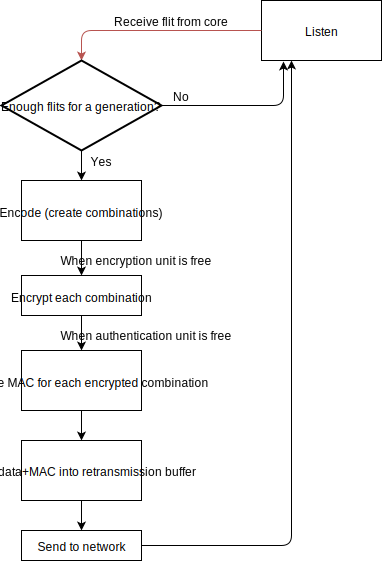
\includegraphics[width=\textwidth]{protocol-flowchart-nc-1}
    \caption[Protocol flow: method 1 coded]{Protocol flow: method 1 coded}
    \label{fig:protchartnc1}
\end{figure}
% uncoded (full explanation), network coded

\subsection{Interwoven Authentication}

\subsection{Full-Generation Authentication}

\section{Routing Strategies}
Mention the perceived/envisioned advantages of adaptive routing (different paths for each flit within the same sender-receiver pair → thanks
to NC enough flits will arrive hopefully even if one path contains a corrupted router).

\subsection{Deterministic XY}
The term \enquote{XY routing} stems directly from the behavior of the routers: flits are only routed along the X axis until they arrive in the column
that the receiver lies in, at which they are routed along the Y axis until reaching the receiver node.
% TODO: figure with a 2D mesh, X and Y arrows on the sides, example path marked for a transmission
\subsection{Dynamic Smart Random}
\subsection{Randomized Oblivious Multi-phase Minimal}
% Both with XY phases and DSR phases
This strategy essentially splits the routing problem into two phases: find a path from sender to proxy node and from proxy to receiver. For each
phase, one of the aforementioned strategies can be applied as is.

\begin{itemize}
    \item Routing Strategies
        \begin{itemize}
            \item Mention routing is general, we are special case of 2D mesh with uniform edge weights → much simpler than arbitrary networks
            \item XY/YX
                \begin{itemize}
                    \item Deterministic path
                    \item Attacker controlling a single router can reliably disrupt communication between certain nodes
                    \item does not distribute flits of a generation across different paths
                \end{itemize}
            \item XY/YX + Valiant
                \begin{itemize}
                    \item Deterministic path only if fixed valiant
                \end{itemize}
            \item Random XorY
            \item Random XorY + Valiant
            \item When writing about this: MANHATTAN DISTANCE (same for XY, YX, random XY, ROMM)
            \item Terminology:
                \begin{itemize}
                    \item Static=deterministic vs. dynamic (one fixed source-destination route or not)
                    \item Oblivious vs. adaptive (take into account network state or not)
                    \item Source routing: source decides a path, this is inserted into flit as metadata
                    \item ROMM is oblivious, use own term RAMM (randomized adaptive multi-phase minimal) for other variant
                    \item ROMM: oblivious, dynamic
                    \item DOR (dimension order routing): oblivious, deterministic
                \end{itemize}
        \end{itemize}
\end{itemize}

\iffalse
\section{Notes}
\begin{itemize}
    \item Encryption/authentication ordering
        \begin{itemize}
            \item Encrypt-then-MAC: best practice. Sequential encrypt/authenticate on sender side, but parallel decrypt/verify
                on receiver side. Advantage: MAC can be computed on receiver side immediately when ciphertext arrives, even when
                MAC flit has not arrived yet (if ARQ is necessary, it can be issued right away)
            \item MAC-then-encrypt: bad. Sequential authenticate/encrypt on sender side and sequential decrypt/verify on receiver
                side.
            \item Encrypt-and-MAC: okay. Parallel encrypt/authenticate on sender side, but sequential decrypt/verify on receiver
                side (overall same latency as Encrypt-then-MAC, but without advantage of fast ARQs)
        \end{itemize}
    \item Uncoded transmission
        \begin{itemize}
            \item no network coding
            \item 2 methods: 1 data flit + 1 MAC flit OR 2 data/MAC split flits
        \end{itemize}
    \item Flit structure
        \begin{itemize}
            \item burst bit, source/target address, mode, address, GID/FID, GEV, payload
            \item mode: define if data/mac/split/arq
        \end{itemize}
    \item Network coded transmission
        \begin{itemize}
            \item Number of flits: G2C3 or G2C4
            \item 3 methods: 1 data flit + 1 MAC flit OR 1 MAC flit per generation OR 2 data/MAC split flits
            \item mention that coded clits are slightly larger due to GEV being embedded → requires wider lanes
        \end{itemize}
    \item ARQs
        \begin{itemize}
            \item Limited number of ARQs per transmission unit (UC: data/MAC pair or split pair, NC: generation)
            \item Timeout of x (e.g. 8) cycles until first ARQ is sent
            \item If limit >1: start larger timeout (→ round-trip of ARQ)
            \item Many different cases, insert some flow diagrams here
            \item The higher the ARQ timeout/limit, the less likely the flit is still in retransmission buffer
            \item → ARQ timeout/limit and retransmission buffer size have to correlate
            \item In the case that we only have 1 ARQ left that we are allowed to send: Wait for any ongoing MAC verifications
                so in case they fail, the flits can be included in the ARQ
        \end{itemize}
\end{itemize}
\fi
